\documentclass{article}

\usepackage[utf8]{inputenc}
\usepackage[T1]{fontenc}
\usepackage[english]{babel}

\usepackage{float}
\usepackage{amsmath}
\usepackage{graphicx}
\usepackage[colorinlistoftodos]{todonotes}
\usepackage{url}
%pour les informations sur un document compilé en PDF et les liens externes / internes
\usepackage{hyperref}
%pour la mise en page des tableaux
\usepackage{array}
\usepackage{tabularx}
\usepackage{setspace}
%modifier la mise en page de l'abstract
\usepackage{abstract}
%police et mise en page (marges) du document
\usepackage[top=4cm, bottom=4cm, left=4cm, right=4cm]{geometry}
%Pour les galerie d'images
\usepackage{subfig}

%====================== INFORMATION ET REGLES ======================

%rajouter les numérotation pour les \paragraphe et \subparagraphe
\setcounter{secnumdepth}{4}
\setcounter{tocdepth}{4}

\hypersetup{							% Information sur le document
pdfauthor = {Premier Auteur,
			Deuxième Auteur,
			Troisième Auteur,
    		Quatrième Auteur},			% Auteurs
pdftitle = {Nom du Projet -
			Sujet du Projet},			% Titre du document
pdfsubject = {Mémoire de Projet},		% Sujet
pdfkeywords = {Tag1, Tag2, Tag3, ...},	% Mots-clefs
pdfstartview={FitH}}					% ajuste la page à la largueur de l'écran

\begin{document}

%régler l'espacement entre les lignes
\newcommand{\HRule}{\rule{\linewidth}{0.5mm}}

%page de garde
\begin{titlepage}
\begin{center}

\textsc{\LARGE \textbf{\'{E}COLE PRATIQUE DES HAUTES ÉTUDES COMMERCIALES}}\\[0.4cm]

% Upper part of the page. The '~' is needed because only works if a paragraph has started.

\includegraphics[width=0.7\textwidth]{ephec.png}~\\[0.4cm]

\texts{\MEDIUM Avenue du Ciseau, 15}\\
\texts{\MEDIUM 1348 Louvain-La-Neuve}\\[1.5cm]

\textsc{\Large }\\[0.5cm]

% Title
\HRule \\[0.4cm]

{\huge \bfseries Development of a car rental management information system \\[0.4cm] }

\HRule \\[0.5cm]

\textbf{Technical defense}

\vspace{1.cm}

% Author and supervisor
\begin{minipage}{0.4\textwidth}
\begin{flushleft} \large
\emph{Author:}\\
Olivier.D NIYONKURU\\
\end{flushleft}
\end{minipage}
\begin{minipage}{0.4\textwidth}
\begin{flushright} \large
\emph{reporter:} \\
\textsc{Louis VAN DORMAEL}
\end{flushright}
\end{minipage}

\vfill

% Bottom of the page
{\large \today}

\end{center}
\end{titlepage}

%page blanche
\newpage

\section{What}

    Before we proceed to describe how this car reservation system will be developed specifically for my client, let's first take a closer look at what’s exactly the car rental booking software. 
    
    \vspace{0.3cm}
    
    From its name, it’s an innovative booking software designed for cars, motorcycles, boats, or trailer rental agencies. It's a secure platform that offers an easy and fast way to smoothly manage car rentals and website reservation systems that makes it an ideal booking software for any rental business.

    \vspace{0.3cm}
    
    Not only does car rental booking software provide him information regarding vehicle maintenance and service tracking one place, but also it will help him to manage billing and invoicing processes more seamlessly.

\section{Problems}

        Car rental reservation software development is in demand among the startups and existing transport companies, which offer autos for rent and deal with multiple orders. 
        
        \vspace{0.3cm}
        
        On the one hand, car rent is a comfortable option for those, who
        
        \vspace{0.3cm}
        
    \begin{itemize}
    
        \item Want a certain level of а mobility and comfort while traveling,
        
        \item Needs a car for a certain period, but does not have the desire or opportunity to buy it.

        \item A lot paper-based work.
        
     \end{itemize}
     
        \vspace{0.3cm}
     
        On the other hand, if you work with people, you know how changeable their plans may be.

\section{Benefits}

  \begin{itemize}
  
	    \item Customer’ self-service,
	    \item 24/7 accepting online reservations and payments,
	    \item Removing the paper-based processes,
	    \item Avoiding risks of overbooking and the factor of          human error,
	    \item Automatic resource management,
	    \item Cuts down on administration processes to improve         business efficiency,
	    \item Making data-driven decisions based on detailed           statistics
	   \item Offers multiple suppliers within one platform to           save users’ time and resources.
	   
	 \end{itemize}

    
\section{Methodology}

    \textbf{Agile.} I will be meeting (virtually or in person) the client every 2 weeks to discuss my progress and to assess his input. 

\section{Planning}

    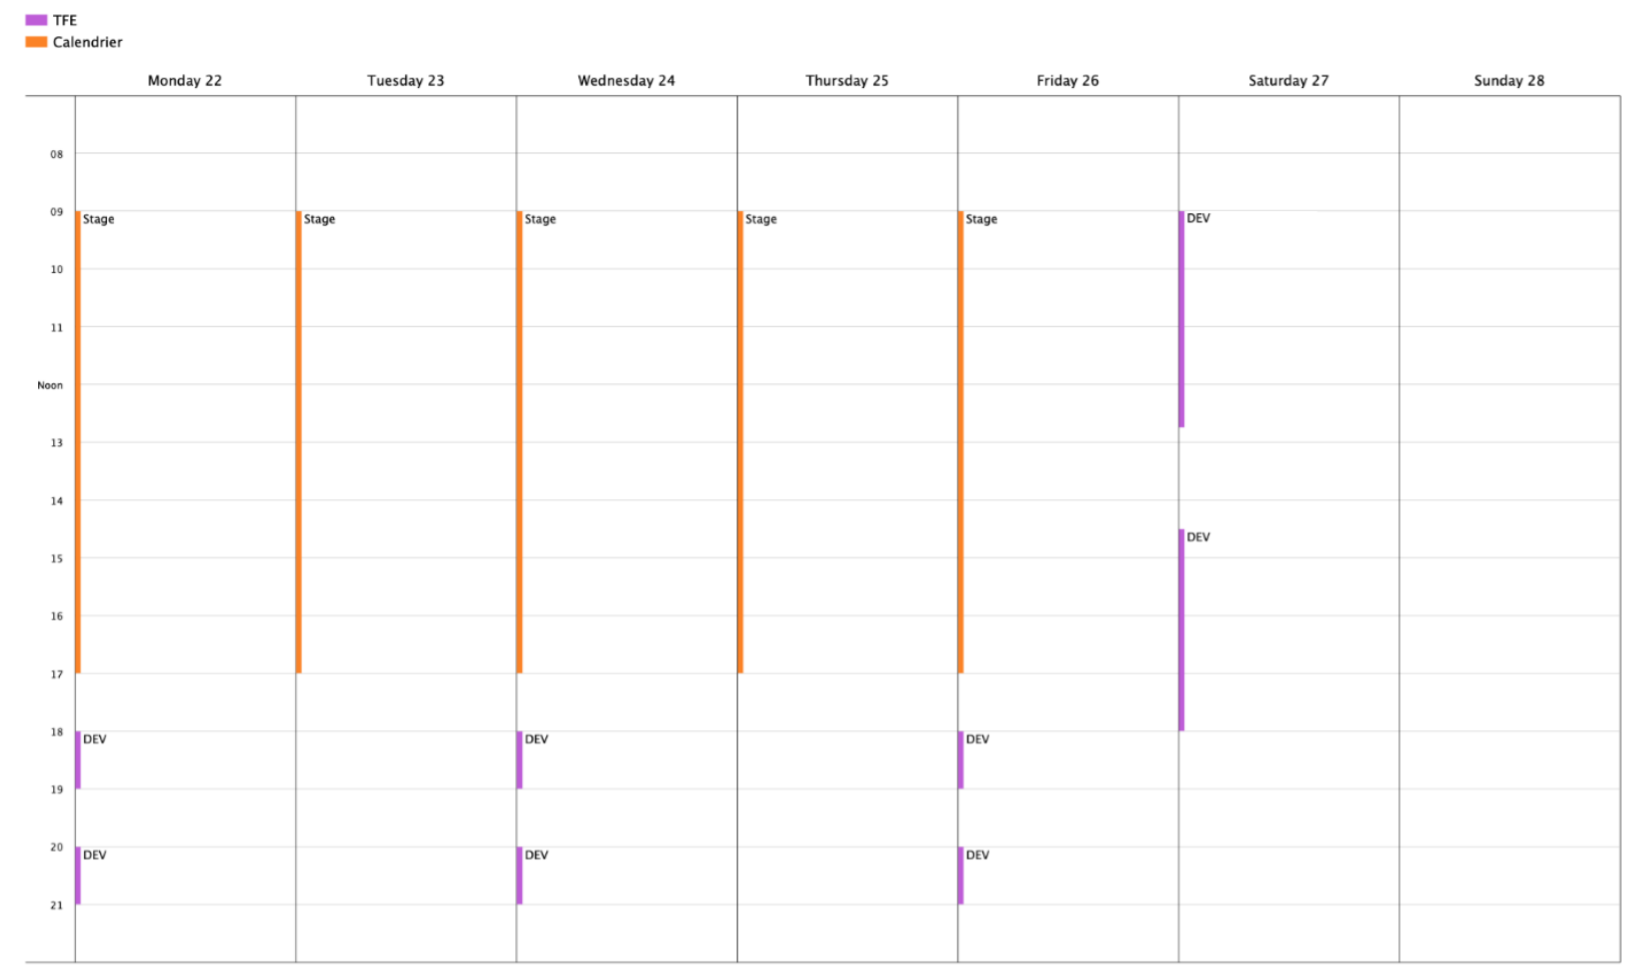
\includegraphics[width=1.2\textwidth]{planning.PNG}~\\[0.2cm]

\pagebreak

\section{Progress}

    \begin{itemize}
        
        \item Contact the client on the technical user stories 
        \item E-R diagram
        \item Relational diagram
        \item Use case diagram 
        \item Class diagram
        \item Git repository
        \item implement the client's user stories in details 
        \item Backend and frontend setup
        \item Deployment setup 

     \end{itemize}
        
\end{document}
